\setcounter{section}{9}
\section{Convergence of Random Variables}

\begin{note}{Prop 10.2}
    Completeness. After $\sum_{k\ge 1}|Y_{k+1}-Y_k|<\infty$ a.s., we have $X:=Y_1+\sum_{k\ge 1}|Y_{k+1}-Y_k|$, so $Y_k\to X$ as $k\to\infty$. We still want to show $d(Y_k,X)\to 0$. Because 
    \[
    d(Y_k,X)=\mathbb{E}[|Y_k-X|\land 1]=\int_{\Omega}(|Y_k(\omega)-X(\omega)|\land 1)\dif\mathbb{P}
    \]
    where $|Y_k(\omega)-X(\omega)|\land 1\le 1$ and $|Y_k(\omega)-X(\omega)|\land 1\to 0\land 1=0$ as $k\to\infty$. By dominated convergence theorem, $d(Y_k,X)\to 0$ a.s.
    \begin{remark}
        With convergence in probability, the dominated convergence theorem permits almost sure convergence along a subsequence.
    \end{remark}
\end{note}

\begin{note}{Prop 10.4}
    In $\mathbb{E}[|X_n-X|^p\mathbf{1}_{\{|X_n-X|>\varepsilon\}}]$, let $f=|X_n-X|^p,g=\mathbf{1}_{\{|X_n-X|>\varepsilon\}}$. We want to get $\mathbb{E}[|\cdot|^r]$. So choose $r/p, r/(r-p)$ as the conjugate exponents,
    \[
    \frac{1}{r/p}+\frac{1}{r/(r-p)}=\frac{p}{r}+\frac{r-p}{r}=1
    \]
\end{note}

\begin{note}{Prop 10.5}
    See p.~27 for the notation of $X^+,X^-$. Since $X=X^+-X^-,|X|=X^++X^-$, we have $|X|-X=2X^-$. And 
    \[
    (X_n-X)^-=(X-X_n)^+=\max(X-X_n,0)\le X
    \]
\end{note}

\begin{figure}[H]
    \centering
    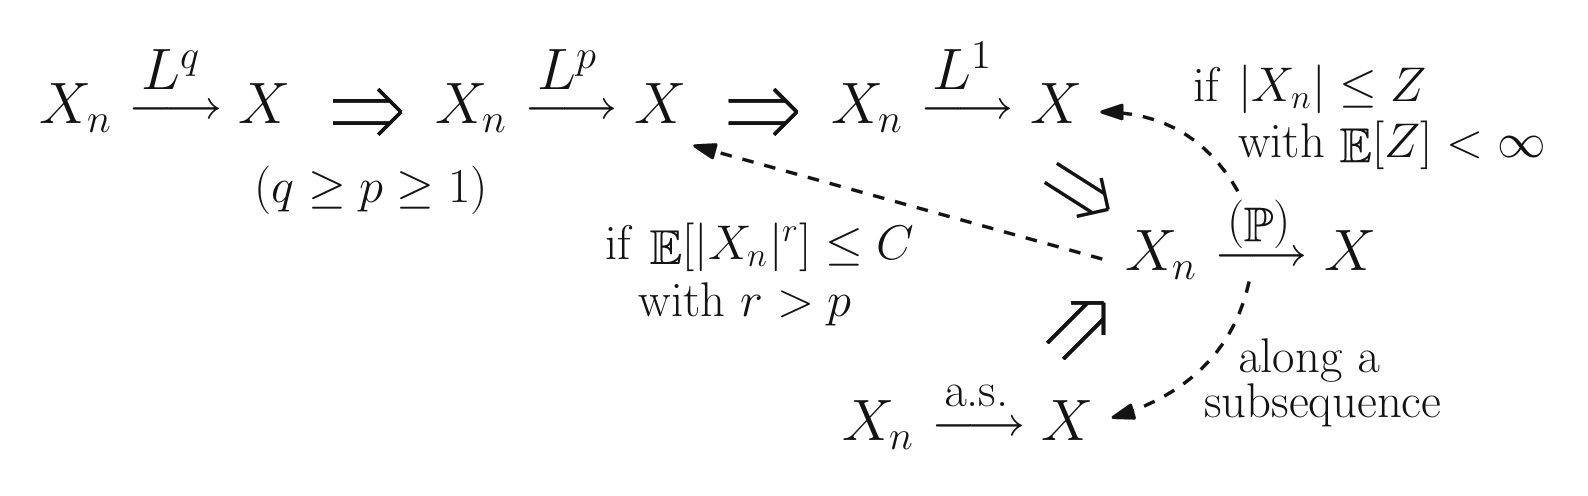
\includegraphics[width=0.65\linewidth]{fig/Fig10-1.png}
    \caption{Relations between the different convergences}
\end{figure}

\begin{note}{Thm 10.6}
    Prove $\sigma(\bigcup_{n\ge 1}\mathcal{D}_n)=\sigma(X_n:n\ge 1)$. 
    \[
    \sigma\!\left(\bigcup_{n=1}^\infty \mathcal{D}_n\right)
= \sigma\!\left(\,\bigcup_{n=1}^\infty \sigma(X_1,\dots,X_n)\right)
    \]
    For each $n\in\mathbb{N}, \sigma(X_1,\dots,X_n)$ is constructed by $\sigma(X_n:n\ge 1)$, so
    \[
    \sigma\!\left(\bigcup_{n=1}^\infty \mathcal{D}_n\right)\subset \sigma(X_n:n\ge 1)
    \]
    Conversely, for each $m\in\mathbb{N}$, $X_m$ is $\mathcal{D}_n$-measurable ($n\ge m$). So
    \[
    \sigma(X_n:n\ge 1)\subset \sigma\!\left(\bigcup_{n=1}^\infty \mathcal{D}_n\right).
    \]
    \begin{remark}
        Use $\mathbb{P}(B)=\mathbb{P}(B)^2$ to give $\mathbb{P}(B)=0\ \text{or}\ 1$ $\impliedby$ $\mathcal{B}_{\infty}$ is independent of itself. If a r.v. $Y$ is $\mathcal{B}_{\infty}$-measurable, $\{Y\le x\}\in\mathcal{B}_{\infty}$ for every $x\in\mathbb{R}$, and $\mathbb{P}(Y\le x)\in\{0,1\}$. See Fig \ref{fig:cdf}.
    \end{remark}
    \begin{figure}[htbp]
        \centering
        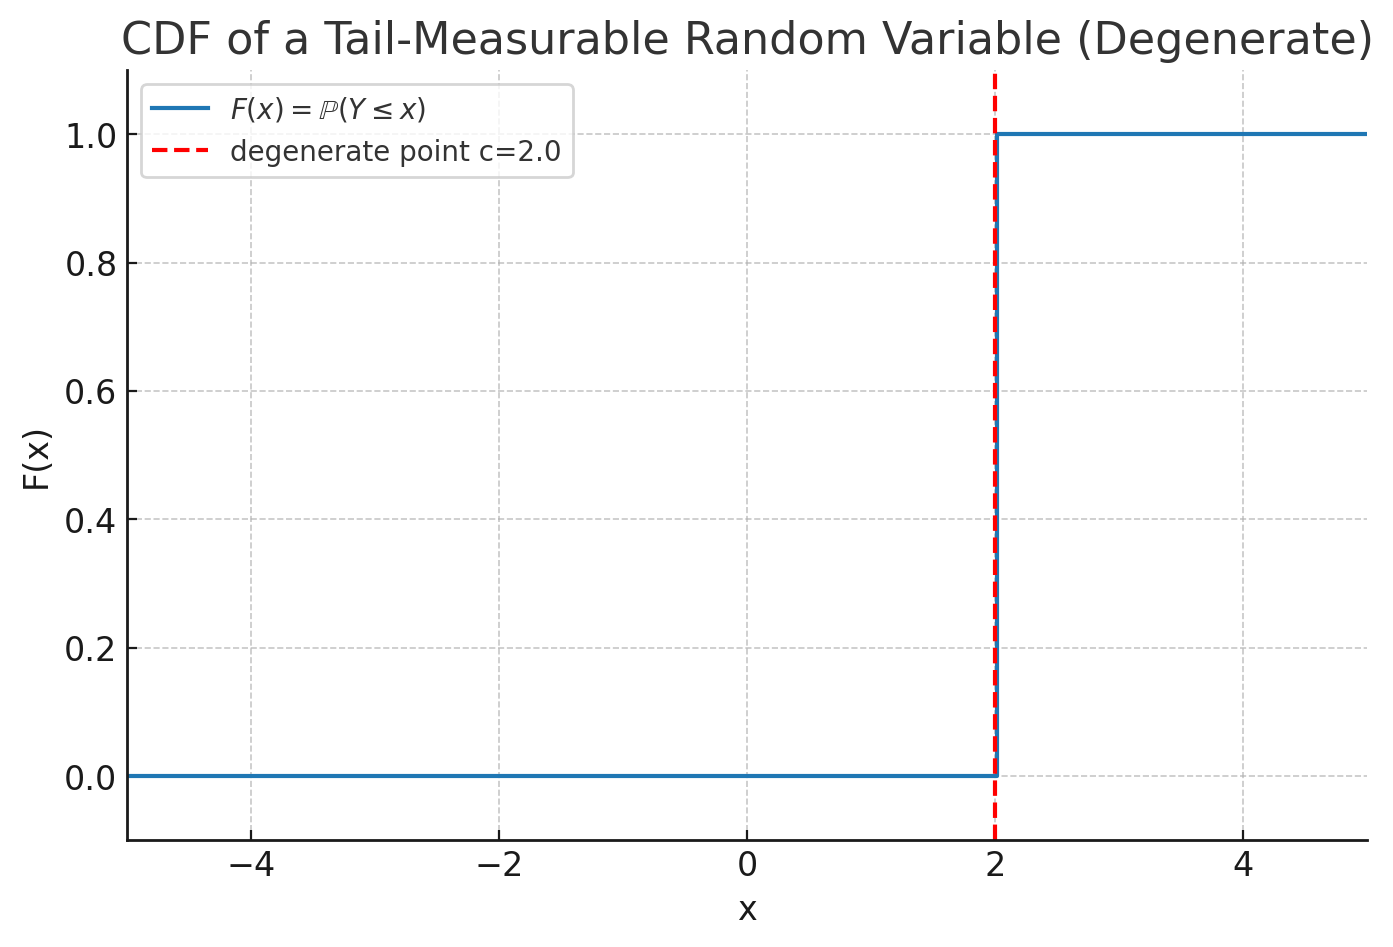
\includegraphics[width=0.65\linewidth]{fig/CDF of a Tail-Measurable Random Variable.png}
        \caption{CDF of a Tail-Measurable Random Variable}
        \label{fig:cdf}
    \end{figure}
\end{note}

\begin{note}{Prop 10.7}
    (1) Let $A_j = \left\{X_{jk+1} = X_{jk+2} = \cdots = X_{jk+k} = 1\right\}$. If this happens, then within that block $S_{(j+1)k}-S_{jk}=k$. So $S_n$ increases by at least $k$. Since $k > 2p$, this jump exceeds the entire width of $[-p, p]$. If even one event $A_j$ occurs, $S_n$ will jump out of $[-p,p]$. Hence, $\exists n,$ such that $A_n$ occurs $\implies$ $S_n>p$. So 
    \[
    \bigcup_{j\ge 1}A_j\subset \left(\left\{-p \leq \inf _{n} S_{n} \leq \sup _{n} S_{n} \leq p\right\}\right)^{c}
    \]
    Because $\mathbb{P}(A_j)=(1/2)^k>0$, $\sum_{j\ge 1}\mathbb{P}(A_j)=\infty$ and $A_j$'s are independent, by Borel-Cantelli lemma, $\mathbb{P}(\limsup A_j)=1\implies A_j$ happens infinitely often.
\end{note}

\begin{note}{p.~210}
    (b) Since $p_n(x)\to p(x)\ \text{a.e.}, p(x)=\liminf_{n\to\infty}p_n(x)$. Use Fatou's lemma. The second inequality derives
    \[
    1-\limsup_{n\to\infty}\int\varphi(x)p_n(x)\dif x\ge 1-\int \varphi(x)p(x)\dif x\implies \limsup_{n\to\infty}\int\varphi(x)p_n(x)\dif x\le \int \varphi(x)p(x)\dif x
    \]
    Combine with the first inequality, 
    \[
    \int \varphi(x)p(x)\dif x\le \liminf_{n\to\infty}\int\varphi(x)p_n(x)\dif x\le
    \limsup_{n\to\infty}\int\varphi(x)p_n(x)\dif x\le \int \varphi(x)p(x)\dif x
    \]
    By squeezing,
    \[
    \lim _{n \rightarrow \infty} \int \varphi(x) p_{n}(x) \mathrm{d} x=\int \varphi(x) p(x) \mathrm{d} x
    \]
\end{note}

\begin{note}{Prop 10.11}
    (i)$\Rightarrow$(ii). Because $0\le\varphi_p\le \mathbf{1}_G$ and $\varphi_p\uparrow \mathbf{1}_G$ pointwise, 
    \[
    \int \varphi_{p} \dif \mu_{n} \leq \int \mathbf{1}_{G} \dif\mu_{n}=\mu_{n}(G) 
    \]

    (ii)$\Leftrightarrow$(iii). Set $F:=G^c, \mu_n(F)=1-\mu_n(G)$. Then use the fact $\liminf(-x)=-\limsup x$. 
\end{note}

\begin{note}{p.~213}
    Consequence. (only if$\Rightarrow$) Since $X_n\xrightarrow{(d)}X$, by property (iv) in Prop 10.11, for $B=(-\infty,x]\in\mathcal{B}(\mathbb{R}^d)$,
    \[
    F_{X_n}(x)=\mu_n((-\infty,x])\to\mu((-\infty,x])=F_X(x)
    \]
    since $\partial B=\bar{B}\setminus B^{\circ}=(-\infty,x]\setminus(-\infty,x)=\{x\}$ and $\mu(\{x\})=0$.

    (if $\Leftarrow$) Let $x_p\downarrow x$. Since $x_p>x, F_{X_n}(x)<F_{X_n}(x_p)$, and let $x_p$ be the points that $F_X$ is continuous. Take limsup,
    \[
    \limsup_{n\to\infty} F_{X_n}(x)\le\limsup_{n\to\infty}F_{X_n}(x_p)=\lim_{n\to\infty}F_{X_n}(x_p)=F_X(x_p)
    \]
    As $p\to\infty, x_p\to x$, so $\limsup_{n\to\infty}F_{X_n}(x)\le F_X(x).$ Now consider liminf. For $x_q\uparrow x, F_{X_n}(q)\le F_{X_n}(x)$,
    \[
    \liminf_{n\to\infty} F_{X_n}(x)\ge\limsup_{n\to\infty}F_{X_n}(x_q)=\lim_{n\to\infty}F_{X_n}(x_q)=F_X(x_q)\to F_X(x-)
    \]
    since $F_X$ is not left-continuous. Consider $\mathbb{P}_{X_n}((a,b))=F_{X_n}(b-)-F_{X_n}(a)$,
    \[
    \liminf_{n\to\infty} \mathbb{P}_{X_n}((a,b)) 
    = \liminf_{n\to\infty} \big( F_{X_n}(b-) - F_{X_n}(a) \big) \geq F_X(b-) - F_X(a) 
    = \mathbb{P}_X((a,b))
    \]
    Because any open subset $G$ can be generated by $(a,b)$, see Exercise 1.1, thus property (ii) in Prop 10.11 holds.
\end{note}

\begin{note}{Thm 10.15}
    For the second part, given 
    \[
    Y_n:=\frac{1}{\sqrt{n}}(X_1+\cdots +X_n)\xrightarrow[n\to\infty]{(d)}\mathcal{N}(\sqrt{n}\mathbb{E}[X_1],\sigma^2)
    \]
    So
    \[
    \begin{aligned}
    \lim_{n\to\infty}\mathbb{P}_{Y_n}(Y_n\in [\sqrt{n}\mathbb{E}[X_1]+a, \sqrt{n}\mathbb{E}[X_1]+b])
    &=\frac{1}{\sigma\sqrt{2\pi}}\int_{\sqrt{n}\mathbb{E}[X_1]+a}^{\sqrt{n}\mathbb{E}[X_1]+b}\exp\left(-\frac{y-\sqrt{n}\mathbb{E}[X_1]}{2\sigma^2}\right)\dif y\\
    &=\frac{1}{\sigma\sqrt{2\pi}}\int_a^b \exp\left(-\frac{y'}{2\sigma^2}\right)\dif y'
    \end{aligned}
    \]
    where $y'=y-\sqrt{n}\mathbb{E}[X_1]$. 

    See (10.4), characteristic function is very useful in transforming random variables.
\end{note}